\begin{savequote}[45mm]
\ascii{Any fool can write code that a computer can understand. Good programmers write code that humans can understand.}
\qauthor{\ascii{- Martin Flower}}
\end{savequote}

\chapter{分布式TensorFlow} 
\label{ch:distributed}

\begin{content}

\end{content}

\section{运行模式}

\begin{content}

TensorFlow实现了两种基本的运行模式:

\begin{enum}
  \eitem{本地模式:\ascii{Client, Master, Worker}部署在同一台机器上,运行在单独的进程上;}
  \eitem{分布式模式:\ascii{Client, Master, Worker}部署在不同机器上,运行在不同的进程上。}
\end{enum}

\subsection{本地模式}

对于本地模式,\ascii{Client}负责计算图的构造,然后通过调用\code{Session.run},启动计算图的执行过程。

\ascii{Master}收到计算图执行消息后,启动计算图的剪枝操作;再将子图传递给\ascii{Worker},然后触发\ascii{Worker}执行子图。

\ascii{Worker}根据本地计算设备资源,再将计算子图进行剪枝,分裂,将子图片段分配在各个计算设备上,最后启动各个计算设备并发地执行子图片段。

因为,\ascii{Client},\ascii{Master},\ascii{Worker}在同一进程内,各服务之间是函数调用关系。

\begin{figure}[!h]
\centering
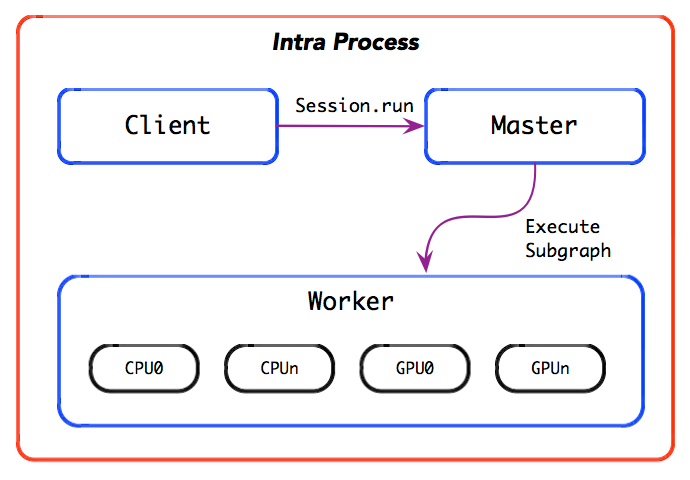
\includegraphics[width=0.9\textwidth]{figures/local.png}
\caption{本地模式}
 \label{fig:local}
\end{figure}

\subsection{分布式模式}

对于分布式模式,\ascii{Client}负责计算图的构造,然后通过调用\code{Session.run},启动计算图的执行过程。

\ascii{Master}进程收到计算图执行消息后,启动计算图的剪枝,分裂,优化等操作;最终将子图分发注册到各个\ascii{Worker}进程,然后触发各个\ascii{Worker}进程执行子图。

\ascii{Worker}进程收到子图注册的消息后,根据本地计算设备资源,再将计算子图进行剪枝,分裂,将子图片段分配在各个计算设备上,最后启动各个计算设备并发地执行子图片段;如果\ascii{Worker}之间存在数据交换,可以通过设备间通信完成交互。

\begin{figure}[!h]
\centering
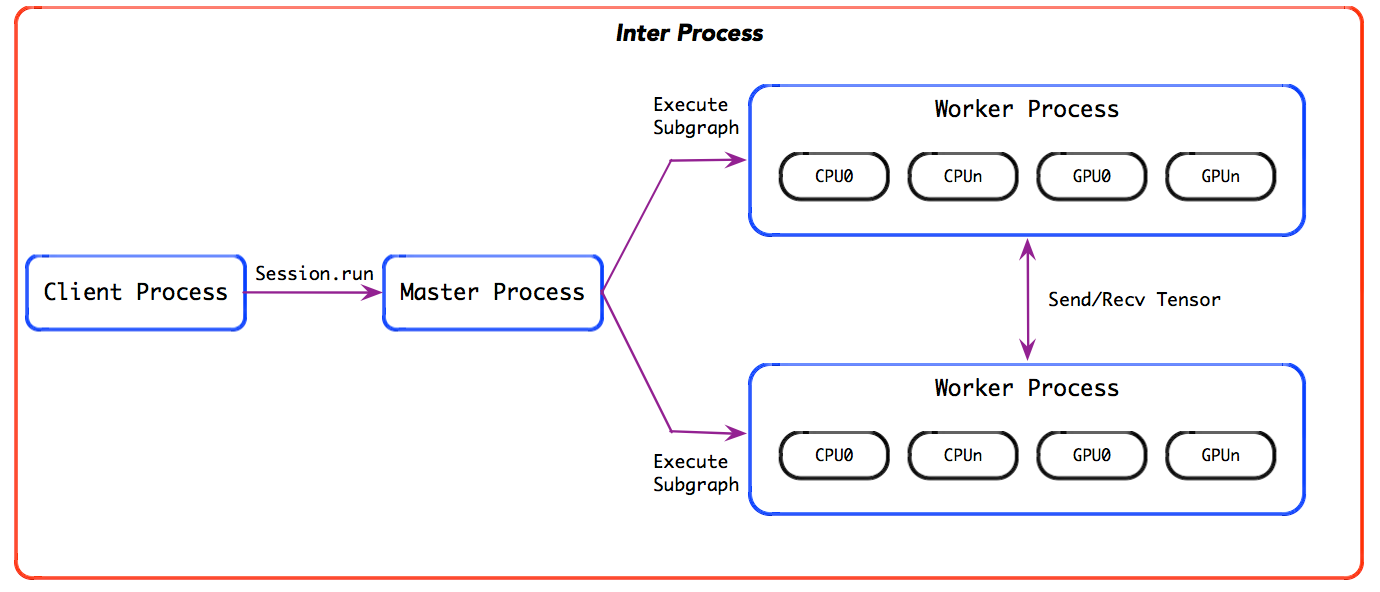
\includegraphics[width=0.9\textwidth]{figures/distributed.png}
\caption{分布式模式}
 \label{fig:distributed}
\end{figure}

\end{content}

\section{领域模型}

\begin{content}

\begin{figure}[!h]
\centering
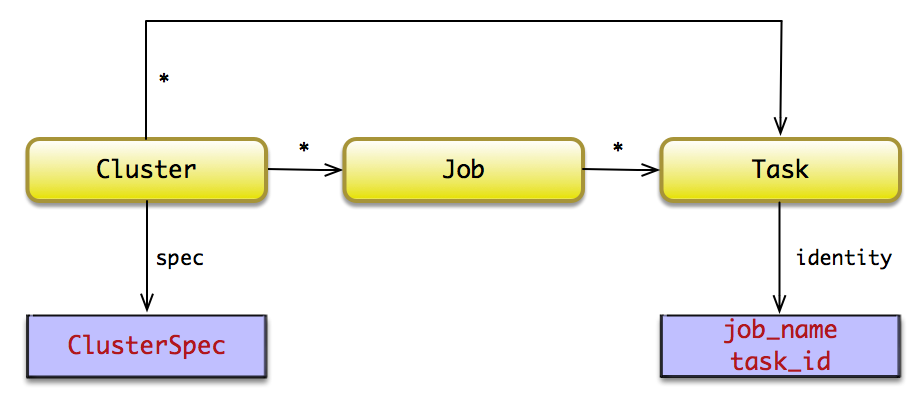
\includegraphics[width=0.9\textwidth]{figures/cc-dist-model.png}
\caption{分布式模式:领域模型}
 \label{fig:cc-dist-model}
\end{figure}

\subsection{Cluster}

一个\ascii{Cluster}可以划分为一个或多个\ascii{Job},一个\ascii{Job}包含一个或多个\ascii{Task}。也就是说,\ascii{TensorFlow}集群是由执行计算图的任务集\ascii{(Task Set)}组成。

每个\ascii{Task}可以独立运行在单独的机器上,也可以在一台机器上运行多个\ascii{Task}(例如,单机多\ascii{CPU},或单机多\ascii{GPU})。

其中,\ascii{Cluster}使用\ascii{ClusterSpec}进行描述,后文详细描述。

\subsection{Job}

将目的相同的\ascii{Task}归类为一个\ascii{Job}。一般地,在分布式深度学习训练过程中,将任务分为两类\ascii{Job}:

\begin{enum}
  \eitem{\ascii{PS}:负责模型参数的存储和更新;}
  \eitem{\ascii{Worker}:负责计算密集型的模型训练和推理。}
\end{enum}

\begin{figure}[!h]
\centering
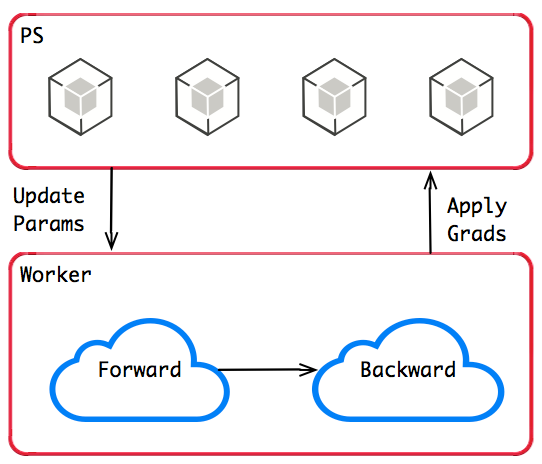
\includegraphics[width=0.6\textwidth]{figures/py-dist-ps-worker.png}
\caption{分布式模式:PS任务与Worker任务}
 \label{fig:py-dist-ps-worker}
\end{figure}

\subsection{Task}

在\ascii{Worker}节点上执行的独立任务。一般地,每个\ascii{Task}启动一个进程,并在其之上运行一个\code{tf.train.Server}实例。

其中,\ascii{Task}使用\ascii{Job}名称与\ascii{Task}索引唯一标识:\code{job\_name:task\_index}。

\subsection{Server}

\ascii{Server}表示\ascii{Task}在运行时的服务进程,它对外提供\ascii{Master Service}服务和\ascii{Worker Service}服务。

\subsection{Master Service}

\ascii{Master Service}是一个\ascii{RPC}服务,客户端通过\ascii{Session}目标(\ascii{target})获取远端的一组分布式的设备集,并执行计算图的计算。

\ascii{Master Service}定义了接入\ascii{Master}的接口定义,即\code{master\_service.proto}中定义的接口;它负责协调和控制多个\ascii{Worker Service}的执行过程。

当\ascii{Client}根据\code{target}接入\ascii{Server}实例,\ascii{Server}扮演了\ascii{Master}的角色,对外提供\ascii{Master Service}服务;其中,\ascii{Client}与\ascii{Master}之间的交互遵循\ascii{Master Service}的接口规范。

\subsection{Worker Service}

\ascii{Worker Service}也是一个\ascii{RPC}服务,负责调度本地设备集执行本地子图。它定义了接入\ascii{Worker}的接口规范,即\code{master\_service.proto}中定义的接口。

\ascii{Master}根据\code{ClusterSpec}信息,找到集群中其他的\ascii{Server}实例,此时这些\ascii{Server}实例将扮演\ascii{Worker}的角色;\ascii{Master}将子图分发给各个\ascii{Worker}节点,并启动各个\ascii{Worker}节点的子图计算的执行过程。

如果\ascii{Worker}之间存在数据依赖,则通过设备间通信完成交互。其中,\ascii{Master}与\ascii{Worker}之间,\ascii{Worker}与\ascii{Worker}之间的交互遵循\ascii{Worker Service}的接口规范。

特殊地,\ascii{Client}与\ascii{Master}可能在同一进程之内;\ascii{Master}与本地的\ascii{Worker}也可能在同一进程中。

\end{content}

\section{组建集群}

\begin{content}

为每个\ascii{Task}创建一个\ascii{Server},并启动相应的\ascii{Server}服务,如此便很容易地组建了一个\ascii{TensorFlow}集群。也就是说,组建\ascii{TensorFlow}集群包括两个基本步骤:

\begin{enum}
  \eitem{创建\code{tf.train.ClusterSpec},描述集群中\ascii{Task}的部署信息,并以\ascii{Job}的方式组织;}
  \eitem{对于每一个\ascii{Task},启动一个\code{tf.train.Server}实例。}
\end{enum}

\subsection{ClusterSpec}

\code{ClusterSpec}描述了集群中\ascii{Task}的部署信息,并以\ascii{Job}的方式组织。一般地,在分布式的执行模式中,为每个\ascii{Task}启动一个进程;因此,\code{ClusterSpec}同时也描述了\ascii{TensorFlow}分布式运行时的进程分布情况。

例如,存在一个\ascii{TensorFlow}集群,它由\code{ps}和\code{worker}两个\ascii{Job}组成。其中,\code{ps}部署在\code{ps0:2222, ps1:2222}上;\code{worker}部署在\code{worker0:2222, worker1:2222, worker2:2222}上。

\begin{leftbar}
\begin{python}
tf.train.ClusterSpec({
  "worker": [
    "worker0:2222",   # /job:worker/task:0
    "worker1:2222",   # /job:worker/task:1
    "worker2:2222"    # /job:worker/task:2
  ],  
  "ps": [
    "ps0:2222",       # /job:ps/task:0
    "ps1:2222"        # /job:ps/task:0
  ]})
\end{python}
\end{leftbar}

在此例中,未显式地指定\ascii{Task}的索引。因此,\ascii{Task}索引在\ascii{Job}的\ascii{Task}集合中从\ascii{0}开始,按序自增的。

\subsection{Protobuf描述}

\begin{leftbar}
\begin{python}
message JobDef {
  string name = 1;
  map<int32, string> tasks = 2;
}

message ClusterDef {
  repeated JobDef job = 1;
}
\end{python}
\end{leftbar}

其中,\code{tasks}的关键字表示\code{task\_index},值表示\code{host:port}。

\end{content}

\section{Server}

\begin{content}

\ascii{Server}是一个基于\ascii{GRPC}的服务器,负责管理本地设备集。它对外提供\ascii{Master Service}服务和\ascii{Worker Service}服务。

\subsection{领域模型}

一般地,一个\ascii{Task}实例上启动一个\ascii{Server}实例。因此,一个\ascii{Server}实例通过\code{job\_name, task\_index}唯一标识,与\ascii{Task}实例一一对应。

另外,一个\ascii{Server}实例通过\code{ClusterSpec}与其他\ascii{Server}实例实现互联。

\begin{figure}[!h]
\centering
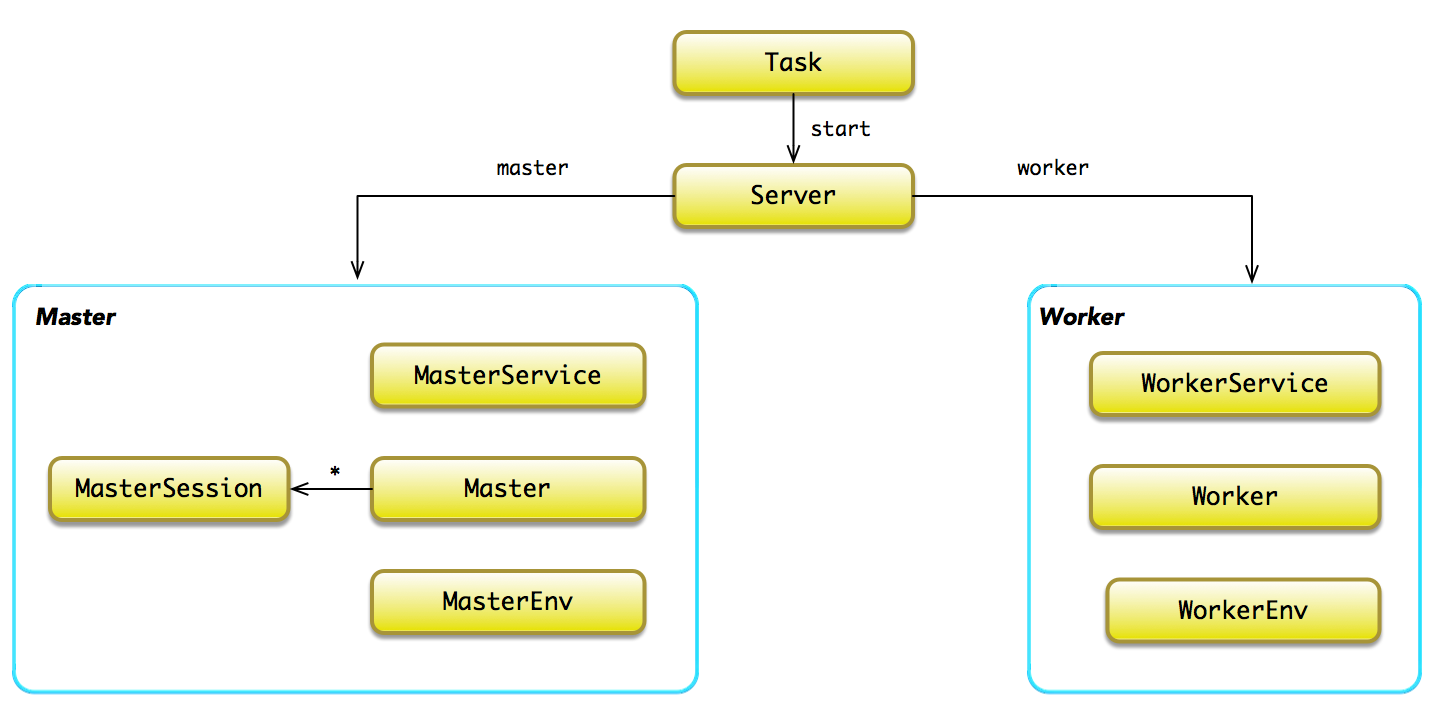
\includegraphics[width=1.0\textwidth]{figures/cc-server-model.png}
\caption{Server架构}
 \label{fig:cc-server-model}
\end{figure}

\subsection{Protobuf描述}

当\code{protocol}为\code{grpc}时,则该\ascii{Server}实例将实现基于\ascii{GRPC}的服务;此外,可以通过\code{ConfigProto}实现运行时的参数配置。

\begin{leftbar}
\begin{python}
message ServerDef {
  ClusterDef cluster = 1;
  
  string job_name = 2;
  int32 task_index = 3;

  ConfigProto default_session_config = 4;
  string protocol = 5;
}
\end{python}
\end{leftbar}

\subsection{服务互联}

一个\ascii{Server}实例通过\code{tf.train.ClusterSpec}与集群中的其他\ascii{Server}实例实现互联。

\begin{figure}[!h]
\centering
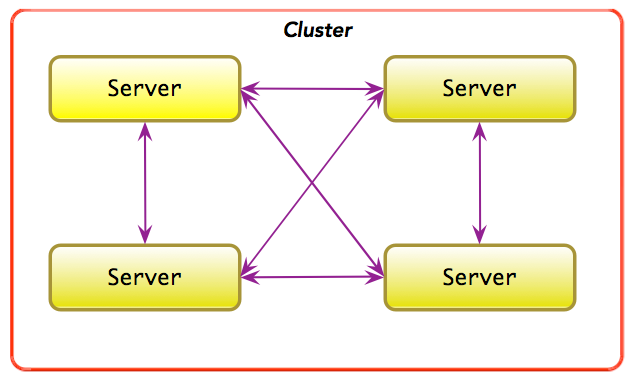
\includegraphics[width=0.8\textwidth]{figures/cc-server-interact.png}
\caption{服务互联}
 \label{fig:cc-server-interact}
\end{figure}

当客户端接入其中一个\ascii{Server},此时它扮演了\ascii{Master}的角色,其他\ascii{Server}则扮演了\ascii{Worker}的角色。在分布式的深度学习训练模式中,存在多个客户端分别接入不同的\ascii{Server}实例。此时,客户端接入的\ascii{Server}实例,同时扮演了\ascii{Master}和\ascii{Worker}的角色。

\begin{figure}[!h]
\centering
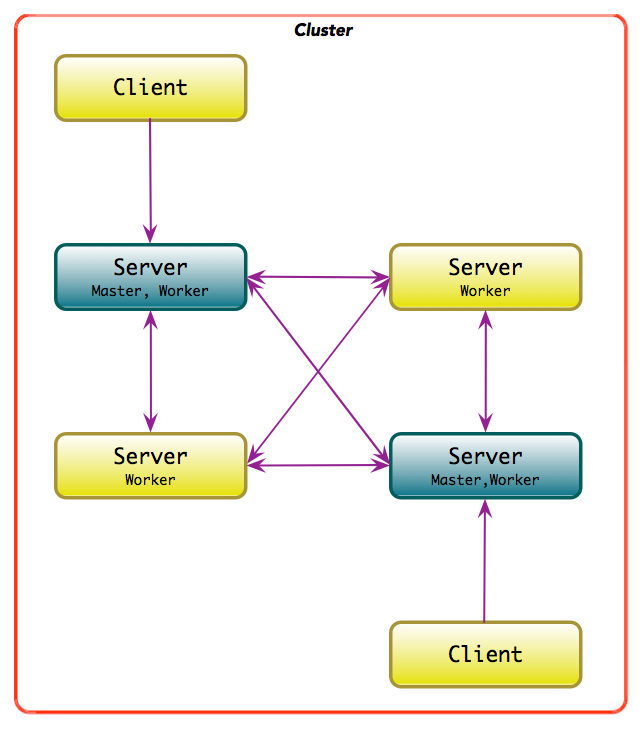
\includegraphics[width=0.8\textwidth]{figures/cc-server-interact-2.png}
\caption{多客户端接入}
 \label{fig:cc-server-interact-2}
\end{figure}

特殊地,\ascii{Client}与\ascii{Master}可以部署在同一个进程内。此时,\ascii{Client}与\ascii{Master}之间的交互更加简单,避免了\ascii{GRPC}的交互。



